% Standard LaTeX document template
%  BE SURE TO PROCESS DOCUMENT TWICE IF IT CONTAINS CROSS-REFERENCES!

\documentclass[12pt]{article}
\usepackage[round]{natbib} %allow to set the bibliography style and
% import the bibliography file. See Bibliography management with
% natbib for more information on
% https://www.sharelatex.com/learn/Bibliography_management_with_natbib.
% See the reference sheet for natbib on
% http://merkel.zoneo.net/Latex/natbib.php.
% Several .bst files can be
% downloaded from http://kinglab.eeb.lsa.umich.edu/pub/biblios/bst/

\usepackage{graphicx,epsfig}
\usepackage{amssymb,amsmath,amsfonts,bm,color,supertabular,longtable,multirow}
\usepackage[colorlinks=true,linkcolor=black,citecolor=black,urlcolor=black]{hyperref}

\setlength{\oddsidemargin}{0in} % left margin, odd pages
\setlength{\evensidemargin}{0in} % left margin, even pages
\setlength{\textwidth}{6.5in} % widtth of text on page
\setlength{\topmargin}{-.3in} % add to default 1 in
\setlength{\headsep}{0in}     % add to default 25pt
\setlength{\textheight}{8.7in}  % height of text on page
\setlength{\parskip}{.1in}            % vertical space between paragraphs
\setcounter{tocdepth}{2}

%\setlength{\parindent}{0in}            % amount of indentation of paragraph


%  newcommands -- more newcommands used in the document.
%  not just in the preamble

\newcommand{\Var}{\mbox{Var}}
\newcommand{\Cov}{\mbox{Cov}}
\newcommand{\E}{\mbox{E}}
\newcommand{\ubeta}{\mbox{\boldmath$\beta$}}
% Independence symbol
\newcommand\independent{\protect\mathpalette{\protect\independenT}{\perp}}
\def\independenT#1#2{\mathrel{\rlap{$#1#2$}\mkern2mu{#1#2}}}


\title{STAT 480 Research Methods\\ Introduction to Latex} 
\author{Ivy Liu\\
School of Mathematics and Statistics\\ Victoria University of Wellington, New Zealand} 
%\date{}  % Add \date{} to make a blank date.


%  main body of document

\begin{document}

% Titlepage
\maketitle

\begin{abstract}
  This course provides students with an opportunity to develop their
  research skills in Mathematics and Statistics, including use of
  library resources, constructing literature reviews, developing
  research questions, writing research proposals, and developing
  skills in oral presentation. The template file gives an introduction
  to LaTeX,
\end{abstract}


% Table of Contents
\tableofcontents


\setlength{\baselineskip}{0.25in} % min space from bottom of one line

                                 % to top of next in a paragraph

                                 % place after \begin{document}



\newpage  % start from a new page
\section{Introduction}

\label{s.intro}


This is the first section of the document. This is the first section of the document. This is the first section of the document.  This is the first section of the document. This is the first section of the document. This is the first section of the document. This is the first section of the document. This is the first section of the document. This is the first section of the document. This is the first section of the document.

In STAT 393, an example shows a set of observations of a {\bf continuous} outcome
variable $y$ on a set of $n$ individuals.
\begin{quote}
{\bf Examples.}  Height, weight, speed, density, ...
\end{quote}
We consider a model:
\begin{equation}
\label{eq:model}
   y_i =\mu + \varepsilon_i, \hspace{.1in} \mbox{where }
   \varepsilon_i \overset{\text{iid}}{\sim} N(0,\sigma^2)\hspace{.1in}
       \text{for } i=1,\ldots,n.
\end{equation}
The General Linear Model is specified as follows:
\[
  {\bf y}_{n\times 1}=
  {X}_{n\times p}\ubeta_{p\times 1}+\bm{\varepsilon}_{n\times 1}
  \hspace{.3in} \bm{\varepsilon}\sim N({\bf 0},\,\sigma^2{I})
\]
Also, $r({X})=p<n$ (${X}$ has full column rank.)  The model (\ref{eq:model}) can be written in the matrix form.  For example,
\begin{eqnarray*}
{\bf y}_{n\times 1} &=&  \left[\begin{array}{c}y_1\\ y_2\\ \vdots\\ y_n\end{array}\right]\\
X_{n\times p}&=&
 \left[\begin{array}{c}1\\ 1\\ \vdots\\ 1\end{array}\right]
\hspace{.1in} \mbox{ and }
\ubeta=\left[ \mu \right ]
\end{eqnarray*}


To estimate $\ubeta$ and $\sigma^2$, for a given set of data ${\bf y}$ and a
design matrix $X$, we want to maximise its likelihood.  STAT 393 shows the method.


\section{Second section}

\label{s.second}

This is the second section of the document. This is the second section of the 
document. In Section \ref{s.intro} on page \pageref{s.intro}, we saw ``This is 
the first section of the document''.

\subsection{Subsection}

\label{ss.a}

This is a subsection in Section \ref{s.second}. This subsection shows how to 
cite papers using a bibliography style.  However, there are many other styles 
available.

\begin{quote}
{\bf Example}

{\em There are a variety of approaches to the modelling of ordinal data
that properly respect the ordinal nature of the data, without the
assumption that the data are continuous.  \cite{Liu05}
 described various proportional odds version
models using adjacent--categories logits, cumulative logits
\citep{McC80}, and continuation--ratio logits \citep{McC89}.}
\end{quote}

\section{Third section}

\label{s.3rd}

We can import pdf files.  For example, Figure \ref{fig:boxplot} shows boxplots. 
If you import pdf files, you need to use pdflatex to 
compile it. If you import ps or eps files, you need to use latex to compile it. 


%\setcounter{figure}{1}  % The next figure will be labeled as Figure 2.
\begin{figure}[htbp] \caption{Box plots}  % always put \caption first and then \label second.
\label{fig:boxplot}
\vspace*{-2in}
\rotatebox{0}{\scalebox{0.8}{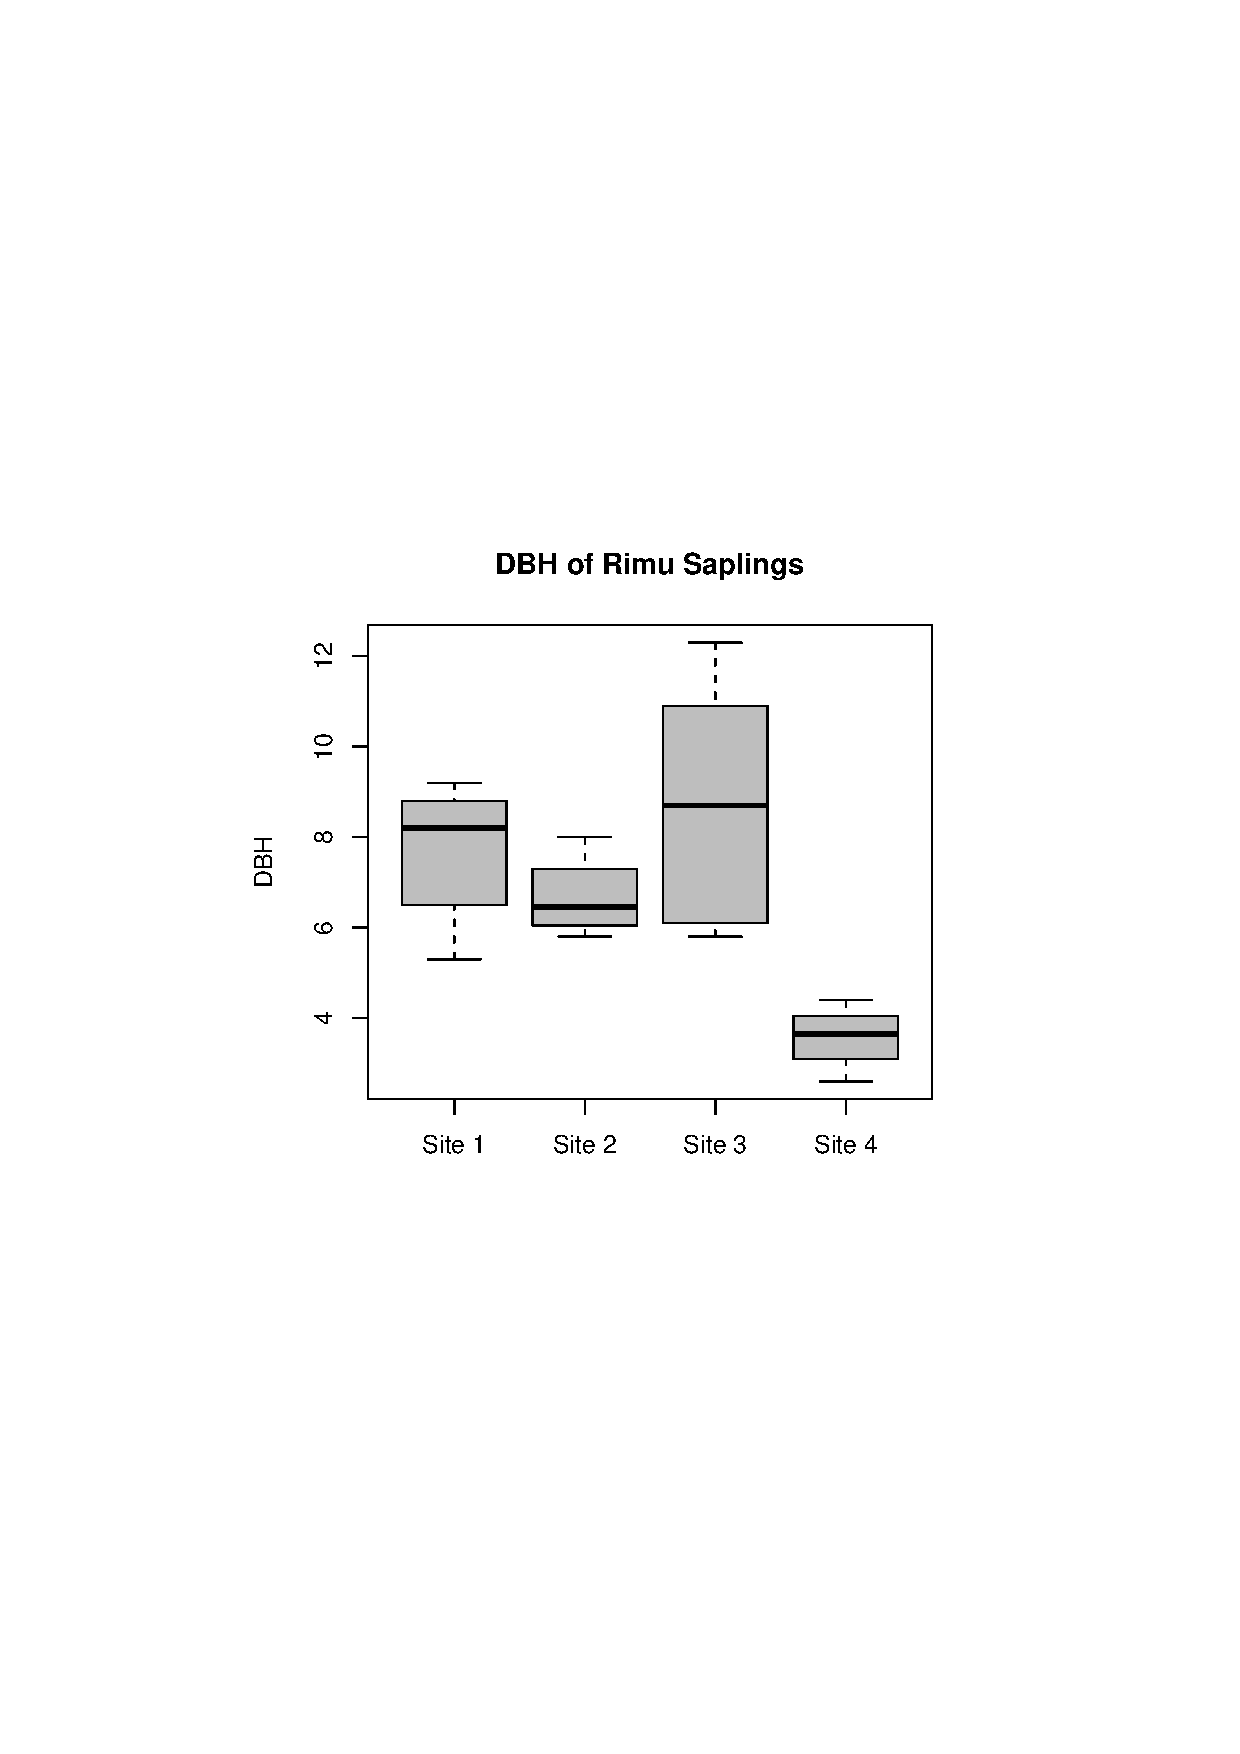
\includegraphics{dbhboxplots.pdf}}}
\end{figure}


\newpage
Table \ref{ta:chi} shows a scanned image.  Also, we can create a table using \verb#\begin{tabular}# as in Table \ref{ta:sample}.

\begin{table}[htbp]
\begin{center}
\caption{Compare nominal and actual $\alpha$-levels for $X^2$ and $G^2$. Table taken from \cite{Fag13}.}
\vspace{.2in}
\label{ta:chi}
\end{center}
\end{table}

\begin{center}
\rotatebox{-90}{\scalebox{0.8}{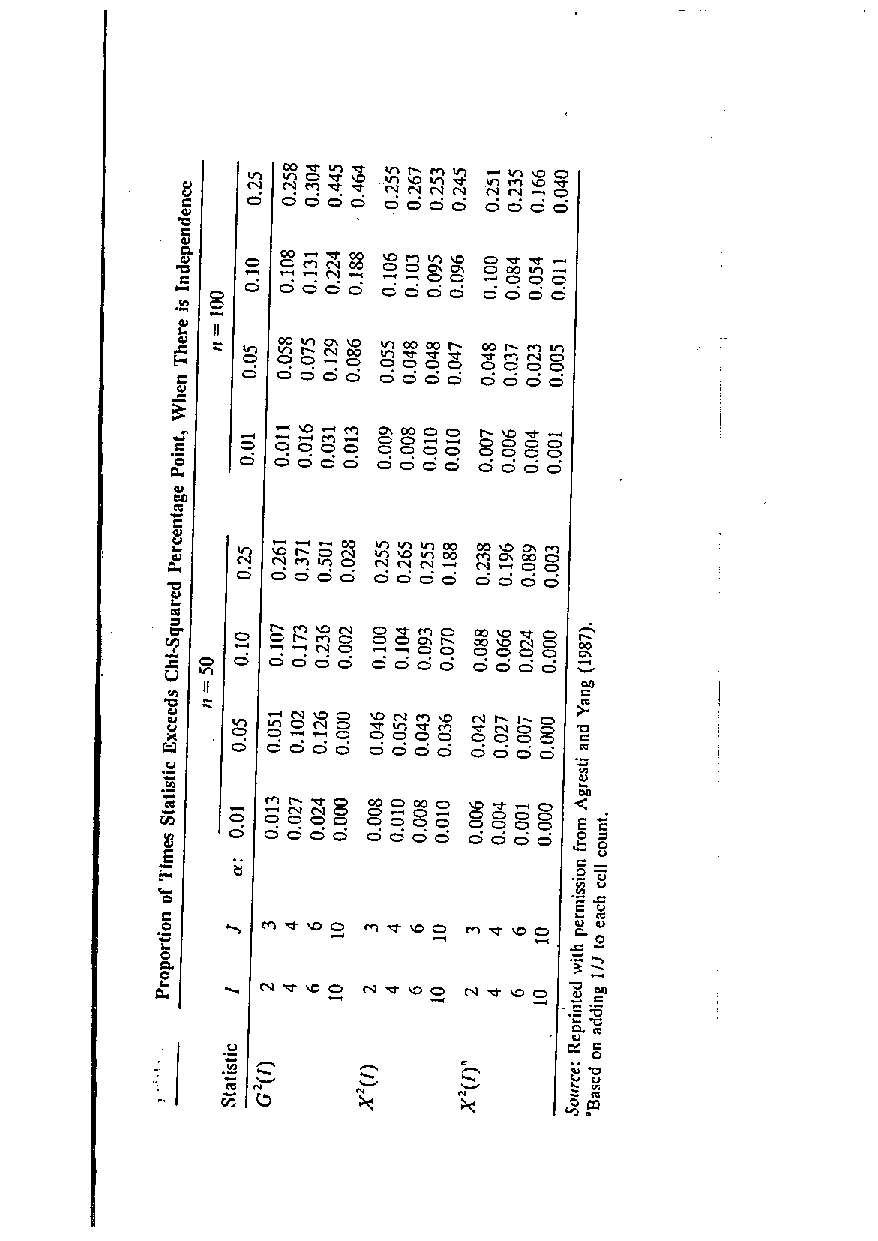
\includegraphics{chisq.pdf}}}
\end{center}


\begin{table}[htbp]
\begin{center}
\caption{Correlation structures}
\vspace{.1in}
\label{ta:sample}
\begin{tabular}{c|c} 
index  & ($R_{ig,12}$,$R_{ig,13}$, $R_{ig,23})$\\
\hline
1 & (-0.1, -0.1, -0.1) \\
2 &  (0.1,  0.1,  0.1) \\
3 &  (0.3,  0.3,  0.3) \\
4 &  (0.5,  0.5,  0.5) \\
5 &  (0.1,  0.3,  0.5) \\
6 &  (0.2,  0.4,  0.6) \\
7 &  (0.1,  0.2,  0.3) \\
8 &  (0.3,  0.4,  0.5)\\
\hline
\end{tabular}
\end{center}
\end{table}

  




\section{Longtable}

\label{s.long}

Here is an example to create a long table. Here is an example to create a long table. Here is an example to create a long table. Here is an example to create a long table. 

Here is an example to create a long table. Here is an example to create a long table. Here is an example to create a long table. Here is an example to create a long table. 


\begin{center}
%% \newpage
\begin{longtable}{|c |c |c |c|}
\caption{Results from the simulation study \label{tab1}}\\
\hline
\multicolumn{1}{|c|}{\textbf{Parameter}} & 
\multicolumn{1}{c|}{\textbf{True value}} & 
\multicolumn{1}{c|}{\textbf{Mean of estimates}} & 
\multicolumn{1}{c|}{\textbf{Std. deviation of estimates}} \\[2mm]
\hline
\endfirsthead
\caption[]{-- continued from previous page} \\
\hline 
\multicolumn{1}{|c|}{\textbf{Parameter}} & 
\multicolumn{1}{c|}{\textbf{True value}} & 
\multicolumn{1}{c|}{\textbf{Mean of estimates}} & 
\multicolumn{1}{c|}{\textbf{Std. deviation of estimates}}  \\[2mm]
\hline
\endhead

\hline \multicolumn{4}{|r|}{{Continued on next page}} \\ \hline
\endfoot

\hline \hline
\endlastfoot
$a_2$ &1.80 & 1.445 & 0.065 \\
$a_3$ &3.60 & 3.031  & 0.110  \\
$b_1$ &2.00 & 2.155  & 0.150 \\  
$b_2$ &1.40 & 1.402  & 0.093 \\
$b_3$ &1.60 & 1.580  & 0.121 \\
$b_4$ &1.30 & 1.297  & 0.104 \\
$b_5$ &1.10 & 1.065  & 0.057 \\
$b_6$ &0.60 & 0.570  & 0.060\\
$\phi_2$ & 0.20 & 0.119 & 0.032 \\
$\rho$ & 0.40 & 0.168   & 0.022\\
$\beta_0(t_0)$ &-0.03 & -0.048 & 0.052 \\
$\beta_0(t_1)$ &-0.70 & -0.236 & 0.107\\
$\beta_0(t_2)$ &-0.70& -0.320 & 0.166\\
$\beta_0(t_3)$ &-0.70& -0.350 & 0.127\\
$\beta_0(t_4)$ &-0.60& -0.214 & 0.159\\
$\beta_0(t_5)$ &-0.70& -0.384 & 0.152\\
$\beta_0(t_6)$ &-1.10& -0.740 & 0.125\\
$\beta_1(t_0)$ &0.10& 0.026 & 0.081 \\
$\beta_1(t_1)$ &0.06& 0.018 & 0.145 \\
$\beta_1(t_2)$ &0.30& 0.207 & 0.185 \\
$\beta_1(t_3)$ &0.30& 0.242 & 0.170 \\
$\beta_1(t_4)$ &0.13& 0.020 & 0.179 \\
$\beta_1(t_5)$ &0.14& 0.136 & 0.234 \\
$\beta_1(t_6)$ &0.70& 0.626 & 0.181 \\
$\delta_0$  & -0.20 & -0.088  & 0.183  \\
$\delta_1$  &-1.00 & -1.207  & 0.456\\
\hline
\end{longtable}
\end{center}




\newpage
%
%\bibliographystyle{harvard}
\bibliographystyle{apalike3}
%\bibliographystyle{abbrv} %this is the same as plainnat but with last name fist 
%\bibliographystyle{unsrtnat}  % Sets the bibliography style
                              % unsrtnat. See the article about
                              % bibliography styles for more
                              % information on
                              % https://www.sharelatex.com/learn/Natbib_bibliography_styles
\bibliography{BIBTEX_GOF} 


\end{document}


